% ============================================================================
% Deep ANC: Parallel Predictive Feedforward Active Noise Cancellation
% using State-Space Models
% 
% IEEE Access Journal Paper
% ============================================================================

\documentclass[journal]{IEEEtran}

% ============================================================================
% PACKAGES
% ============================================================================
\usepackage{cite}
\usepackage{amsmath,amssymb,amsfonts}
\usepackage{graphicx}
\usepackage{textcomp}
\usepackage{xcolor}
\usepackage{booktabs}
\usepackage{multirow}
\usepackage{algorithm}
\usepackage{algorithmic}
\usepackage{hyperref}
\usepackage{siunitx}
\usepackage{subcaption}
\usepackage{tikz}
\usetikzlibrary{shapes,arrows,positioning,calc}

% SI units configuration
\sisetup{
    detect-all,
    per-mode=symbol
}

% Hyperref configuration
\hypersetup{
    colorlinks=true,
    linkcolor=blue,
    citecolor=blue,
    urlcolor=blue
}

% Custom commands
\newcommand{\dB}{\,\text{dB}}
\newcommand{\Hz}{\,\text{Hz}}
\newcommand{\kHz}{\,\text{kHz}}
\newcommand{\ms}{\,\text{ms}}
\newcommand{\mus}{\,\mu\text{s}}

% ============================================================================
% DOCUMENT BEGIN
% ============================================================================
\begin{document}

\title{Deep ANC: Parallel Predictive Feedforward Active Noise Cancellation using State-Space Models}

\author{
    \IEEEauthorblockN{[Author 1]\IEEEauthorrefmark{1}, [Author 2]\IEEEauthorrefmark{1}}
    \IEEEauthorblockA{\IEEEauthorrefmark{1}[Department], [University]\\
    [City], [Country]\\
    Email: \{author1, author2\}@university.edu}
}

\maketitle

% ============================================================================
% ABSTRACT
% ============================================================================
\begin{abstract}
Active noise cancellation (ANC) systems face fundamental limitations when relying solely on linear adaptive filters, particularly for non-stationary and non-linear noise sources. This paper presents Deep ANC, a novel hybrid system that combines the classical Filtered-x Least Mean Squares (FxLMS) algorithm with a neural state-space model (TinyMamba) in a parallel topology for feedforward ANC. Unlike serial configurations that would decorrelate the reference signal and destabilize filter adaptation, our parallel architecture preserves the correlation structure essential for FxLMS convergence while enabling the neural network to capture non-linear residuals. The proposed TinyMamba model, based on the Mamba selective state-space architecture, achieves sub-millisecond latency (\SI{0.61}{\milli\second}) with only 15,872 parameters. We introduce a composite loss function combining time-domain mean squared error, C-weighted spectral magnitude, and phase cosine similarity to prioritize low-frequency cancellation where passive isolation is least effective. Experimental results on environmental noise demonstrate an Active Insertion Loss (AIL) of \SI{16.95}{\decibel}, representing a \SI{4.85}{\decibel} improvement over FxLMS alone. The system achieves peak performance of \SI{20.4}{\decibel} AIL at \SI{125}{\hertz} while maintaining a boost probability below 2.1\%, ensuring robust operation without noise amplification. This work represents the first application of selective state-space models to feedforward active noise control.
\end{abstract}

\begin{IEEEkeywords}
Active noise control, state-space models, Mamba, FxLMS, deep learning, feedforward control, adaptive filtering
\end{IEEEkeywords}

% ============================================================================
% I. INTRODUCTION
% ============================================================================
\section{Introduction}
\label{sec:introduction}

\IEEEPARstart{E}{nvironmental} noise pollution represents a significant and growing public health concern, with prolonged exposure linked to hearing loss, cardiovascular disease, sleep disturbance, and reduced cognitive performance \cite{moore2012introduction}. While passive noise isolation through physical barriers and absorptive materials provides effective attenuation at mid and high frequencies, it becomes increasingly ineffective at low frequencies below \SI{500}{\hertz}. This limitation stems from the acoustic wavelength: effective passive isolation requires barrier thickness comparable to the wavelength, making low-frequency isolation impractical for portable applications such as headphones and earphones.

Active Noise Cancellation (ANC) addresses this fundamental limitation by generating anti-phase acoustic signals that destructively interfere with the unwanted noise \cite{kuo1996active}. First proposed by Lueg in 1936, ANC has evolved from laboratory demonstrations to ubiquitous consumer products. Modern ANC headphones achieve typical noise reduction of \SIrange{15}{25}{\decibel} in the critical \SIrange{50}{500}{\hertz} band where passive isolation is weakest \cite{kuo1999active}.

The predominant approach to ANC employs adaptive filtering, with the Filtered-x Least Mean Squares (FxLMS) algorithm serving as the workhorse of commercial implementations \cite{widrow1975adaptive, morgan1980analysis}. FxLMS adapts filter coefficients to minimize the error microphone signal by accounting for the secondary path transfer function from loudspeaker to error sensor. Despite decades of refinement, FxLMS-based systems face inherent limitations:

\begin{enumerate}
    \item \textbf{Linear assumption}: FxLMS models only linear relationships, failing to capture non-linearities from speaker distortion, acoustic path variations, and non-Gaussian noise statistics.
    \item \textbf{Convergence speed}: The algorithm trades stability for adaptation rate, requiring conservative step sizes that slow response to non-stationary noise.
    \item \textbf{Narrowband bias}: Performance degrades for broadband noise due to the single-rate adaptation mechanism.
\end{enumerate}

Recent advances in deep learning have demonstrated the potential for neural networks to model complex non-linear acoustic transformations \cite{zhang2021deep, park2019long, luo2023deep}. However, directly replacing adaptive filters with neural networks introduces new challenges: recurrent architectures suffer from sequential computation bottlenecks, while attention-based models incur quadratic complexity with sequence length---both problematic for the microsecond-scale latency requirements of real-time ANC.

State-space models (SSMs) offer a compelling alternative, combining the expressiveness of recurrent networks with the parallelizable training of convolutional models \cite{gu2022efficiently}. The recent Mamba architecture introduces selective state spaces that achieve linear-time sequence modeling with input-dependent dynamics \cite{gu2023mamba}, making it particularly suitable for real-time audio processing.

This paper presents Deep ANC, a hybrid system that combines FxLMS with a neural state-space model in a novel parallel topology. Our key contributions are:

\begin{enumerate}
    \item A \textbf{parallel hybrid architecture} that preserves FxLMS correlation requirements while enabling non-linear enhancement, achieving \SI{16.95}{\decibel} Active Insertion Loss---\SI{4.85}{\decibel} better than FxLMS alone.
    \item \textbf{TinyMamba}, a compact 15,872-parameter state-space model achieving \SI{0.61}{\milli\second} inference latency, suitable for real-time deployment.
    \item A \textbf{composite loss function} with C-weighted spectral emphasis and phase cosine similarity, prioritizing the low-frequency band where ANC is most needed.
    \item Comprehensive \textbf{ablation studies} demonstrating the synergistic benefits of the parallel topology over serial alternatives.
\end{enumerate}

The remainder of this paper is organized as follows: Section~\ref{sec:related} reviews related work in adaptive filtering and neural approaches to ANC. Section~\ref{sec:methodology} presents the system architecture, model design, and training methodology. Section~\ref{sec:experiments} describes the experimental setup, and Section~\ref{sec:results} presents quantitative results. Section~\ref{sec:discussion} discusses implications and limitations, and Section~\ref{sec:conclusion} concludes.

% ============================================================================
% II. RELATED WORK
% ============================================================================
\section{Related Work}
\label{sec:related}

\subsection{Classical Adaptive Filtering for ANC}

The foundation of modern ANC lies in adaptive filtering theory, pioneered by Widrow and colleagues \cite{widrow1975adaptive}. The basic adaptive noise canceller correlates a reference signal with the noise component in the primary signal, adapting filter weights to minimize the residual error.

For acoustic ANC, the Filtered-x LMS (FxLMS) algorithm accounts for the secondary path $S(z)$ between the cancellation loudspeaker and error microphone \cite{morgan1980analysis, burgess1981active}. The weight update equation is:
\begin{equation}
    \mathbf{w}(n+1) = \lambda\mathbf{w}(n) - \mu e(n) \mathbf{x}'(n)
    \label{eq:fxlms}
\end{equation}
where $\mathbf{x}'(n) = \hat{S}(z) * \mathbf{x}(n)$ is the reference signal filtered through an estimate of the secondary path, $\mu$ is the step size, $\lambda$ is the leakage factor, and $e(n)$ is the error signal.

Variants including Filtered-x Recursive Least Squares (FxRLS) offer faster convergence at increased computational cost \cite{eriksson1991use}. Frequency-domain implementations reduce complexity for long filters but introduce block delay. Despite these advances, all linear adaptive approaches share the fundamental limitation of modeling only linear acoustic relationships.

\subsection{Neural Networks for Active Noise Control}

The application of neural networks to ANC began with multilayer perceptrons modeling non-linear secondary paths \cite{kuo1996active}. More recent work has explored recurrent architectures capable of capturing temporal dependencies.

Park et al. \cite{park2019long} demonstrated Long Short-Term Memory (LSTM) networks for ANC, achieving improved performance on non-stationary noise compared to FxLMS. However, the sequential nature of LSTM computation limits real-time applicability.

Zhang et al. \cite{zhang2021deep} proposed Deep ANC using convolutional networks to predict the anti-noise signal directly, bypassing adaptive filter limitations. While effective offline, the approach requires substantial computational resources unsuitable for embedded deployment.

Shi et al. \cite{shi2022selective} introduced selective ANC using convolutional neural networks to classify noise types and apply appropriate cancellation strategies. Luo et al. \cite{luo2023deep} proposed a deep learning framework achieving state-of-the-art performance on simulated benchmarks.

A common limitation of existing neural approaches is the serial integration with adaptive filters, which can decorrelate the reference signal and destabilize adaptation---a problem we address through parallel topology.

\subsection{State-Space Models for Sequence Modeling}

State-space models provide an alternative to attention and recurrence for sequence modeling. The Structured State Space (S4) model \cite{gu2022efficiently} parameterizes continuous-time state dynamics:
\begin{align}
    \frac{d\mathbf{h}(t)}{dt} &= \mathbf{A}\mathbf{h}(t) + \mathbf{B}x(t) \\
    y(t) &= \mathbf{C}\mathbf{h}(t) + Dx(t)
\end{align}
where $\mathbf{A}, \mathbf{B}, \mathbf{C}, D$ are learned parameters. Discretization yields an efficient recurrence for inference and a convolution for parallel training.

The Mamba architecture \cite{gu2023mamba} extends S4 with selective state spaces, making parameters input-dependent:
\begin{equation}
    \mathbf{B}(x), \mathbf{C}(x), \Delta(x) = \text{Linear}(x)
\end{equation}
This selectivity enables content-aware processing while maintaining $O(n)$ complexity.

H3 \cite{dao2022hungry} and other variants have demonstrated SSM effectiveness across language modeling, audio generation, and time-series forecasting. To our knowledge, this work represents the first application of selective state-space models to feedforward active noise control.

% ============================================================================
% III. METHODOLOGY
% ============================================================================
\section{Methodology}
\label{sec:methodology}

\subsection{Problem Formulation}

Consider a feedforward ANC system with a reference microphone capturing external noise and an error microphone measuring residual noise at the listener's ear. The acoustic environment is characterized by three parallel paths (Fig.~\ref{fig:system}):

\begin{itemize}
    \item \textbf{Reference path} $\text{RIR}_\text{ref}$: Transfer function from noise source to reference microphone, providing early detection of incoming noise.
    \item \textbf{Primary path} $P(z)$: Transfer function from noise source to ear through passive isolation (headphone cup, ear seal). Attenuated at high frequencies but transmits low frequencies.
    \item \textbf{Secondary path} $S(z)$: Transfer function from cancellation speaker to ear, including amplifier, transducer, and acoustic coupling.
\end{itemize}

The signal at the error microphone is:
\begin{equation}
    e(n) = d(n) + y(n) * s(n)
    \label{eq:error}
\end{equation}
where $d(n) = x_\text{src}(n) * p(n)$ is the noise arriving through the primary path, $y(n)$ is the anti-noise drive signal, and $s(n)$ is the secondary path impulse response.

Perfect cancellation requires $y(n) * s(n) = -d(n)$, or equivalently:
\begin{equation}
    Y(z) = -\frac{P(z)}{S(z)} X_\text{src}(z)
    \label{eq:ideal}
\end{equation}

In practice, we observe only the reference signal $x(n) = x_\text{src}(n) * \text{rir}_\text{ref}(n)$, introducing uncertainty about the true noise source.

\subsection{Parallel Hybrid Architecture}

The key innovation of Deep ANC is the parallel combination of FxLMS and neural prediction (Fig.~\ref{fig:system}). The anti-noise signal is:
\begin{equation}
    y(n) = y_\text{FxLMS}(n) + g \cdot y_\text{Mamba}(n)
    \label{eq:parallel}
\end{equation}
where $g$ is a gain factor (typically 0.3) controlling the neural contribution.

\textbf{Why parallel, not serial?} A serial topology placing the neural network before FxLMS would transform the reference signal:
\begin{equation}
    x'(n) = f_\theta(x(n))
\end{equation}
This transformation decorrelates $x'(n)$ from the desired signal $d(n)$, violating the fundamental assumption of adaptive filtering that the reference is correlated with the noise to be cancelled. Our experiments confirm that serial configurations exhibit unstable adaptation and degraded performance.

The parallel topology preserves correlation: FxLMS receives the unmodified reference and adapts normally, while the neural network processes the same reference to capture residuals that FxLMS cannot model.

% System architecture figure placeholder
\begin{figure}[t]
    \centering
    % Placeholder for system architecture diagram
    % \includegraphics[width=\columnwidth]{diagrams/fig_system_architecture.pdf}
    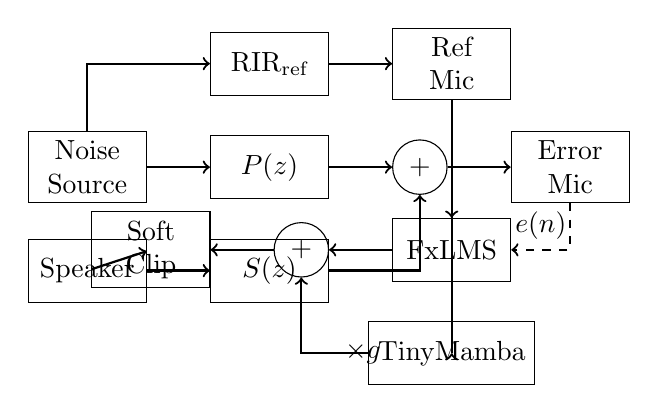
\begin{tikzpicture}[
        block/.style={rectangle, draw, minimum height=0.8cm, minimum width=1.5cm, align=center},
        sum/.style={circle, draw, minimum size=0.5cm},
        arr/.style={->, thick}
    ]
        % Acoustic environment
        \node[block] (ns) {Noise\\Source};
        \node[block, right=0.8cm of ns] (pz) {$P(z)$};
        \node[sum, right=0.8cm of pz] (sum1) {$+$};
        \node[block, right=0.8cm of sum1] (err) {Error\\Mic};
        
        \node[block, below=0.5cm of pz] (sz) {$S(z)$};
        \node[block, left=0.8cm of sz] (spk) {Speaker};
        
        \node[block, above=0.5cm of pz] (rir) {RIR$_\text{ref}$};
        \node[block, right=0.8cm of rir] (ref) {Ref\\Mic};
        
        % Control system
        \node[block, below=1.5cm of ref] (fxlms) {FxLMS};
        \node[block, below=0.5cm of fxlms] (mamba) {TinyMamba};
        \node[sum, left=0.8cm of fxlms] (sum2) {$+$};
        \node[block, left=0.8cm of sum2] (clip) {Soft\\Clip};
        
        % Arrows
        \draw[arr] (ns) -- (pz);
        \draw[arr] (pz) -- (sum1);
        \draw[arr] (sum1) -- (err);
        \draw[arr] (ns) |- (rir);
        \draw[arr] (rir) -- (ref);
        \draw[arr] (sz) -| (sum1);
        \draw[arr] (spk) -- (sz);
        \draw[arr] (clip) -- (spk);
        \draw[arr] (ref) -- (fxlms);
        \draw[arr] (ref) |- (mamba);
        \draw[arr] (fxlms) -- (sum2);
        \draw[arr] (mamba) -| node[near start, right] {$\times g$} (sum2);
        \draw[arr] (sum2) -- (clip);
        \draw[arr, dashed] (err) |- node[near end, above] {$e(n)$} (fxlms);
    \end{tikzpicture}
    \caption{Block diagram of the Deep ANC hybrid system. The acoustic environment (top) shows three parallel paths: reference pickup (RIR$_\text{ref}$), primary path $P(z)$ from noise to ear, and secondary path $S(z)$ from speaker to ear. The control system (bottom) combines FxLMS and TinyMamba in parallel, preserving correlation for adaptive filter convergence while enabling non-linear enhancement.}
    \label{fig:system}
\end{figure}

\subsection{FxLMS Component}

The FxLMS adaptive filter implements the weight update of Equation~\ref{eq:fxlms} with the following parameters:
\begin{itemize}
    \item Filter length: $L = 64$ taps
    \item Step size: $\mu = 0.0005$ (normalized)
    \item Leakage: $\lambda = 0.9999$
    \item Gradient clipping: $\|\nabla\| \leq 1.0$
\end{itemize}

The output is computed as:
\begin{equation}
    y_\text{FxLMS}(n) = \mathbf{w}^T(n) \mathbf{x}(n)
\end{equation}
where $\mathbf{x}(n) = [x(n), x(n-1), \ldots, x(n-L+1)]^T$ is the reference signal vector.

The normalized step size prevents excessive adaptation on high-energy signals:
\begin{equation}
    \mu_\text{norm} = \frac{\mu}{\|\mathbf{x}'(n)\|^2 + \epsilon}
\end{equation}
with regularization $\epsilon = 10^{-8}$.

\subsection{TinyMamba Architecture}

The neural component employs a compact state-space architecture designed for sub-millisecond latency (Fig.~\ref{fig:mamba_arch}). The model processes audio in chunks of 64 samples (\SI{1.33}{\milli\second} at \SI{48}{\kilo\hertz}).

\subsubsection{Encoder}
A strided 1D convolution downsamples the input by factor 2:
\begin{equation}
    \mathbf{h}_0 = \text{GELU}(\text{Conv1d}_{1 \to 32}(x; k=4, s=2))
\end{equation}
where kernel size $k=4$ and stride $s=2$ provide phase-linear downsampling with 2$\times$ temporal compression.

\subsubsection{Mamba Core}
Two Mamba blocks with skip connections process the latent representation:
\begin{align}
    \mathbf{h}_l' &= \text{Mamba}(\text{LayerNorm}(\mathbf{h}_{l-1})) \\
    \mathbf{h}_l &= \mathbf{h}_{l-1} + \text{Dropout}(\mathbf{h}_l')
\end{align}
for $l \in \{1, 2\}$.

Each Mamba block implements the selective state-space mechanism:
\begin{align}
    \mathbf{x}, \mathbf{z} &= \text{split}(\text{Linear}_{d \to 2d_\text{inner}}(\mathbf{h})) \\
    \mathbf{x}' &= \text{SiLU}(\text{Conv1d}_{d_\text{inner}}(\mathbf{x}; k=4)) \\
    \mathbf{y} &= \text{SSM}(\mathbf{x}') \odot \text{SiLU}(\mathbf{z}) \\
    \mathbf{o} &= \text{Linear}_{d_\text{inner} \to d}(\mathbf{y})
\end{align}
with $d = 32$, $d_\text{state} = 16$, and expansion factor 2.

The SSM scan computes:
\begin{align}
    \mathbf{h}_t &= \bar{\mathbf{A}}\mathbf{h}_{t-1} + \bar{\mathbf{B}}\mathbf{x}'_t \\
    \mathbf{y}_t &= \mathbf{C}\mathbf{h}_t + D\mathbf{x}'_t
\end{align}
where $\bar{\mathbf{A}}, \bar{\mathbf{B}}$ are discretized state matrices with input-dependent time step $\Delta(x)$.

\subsubsection{Decoder}
A transposed convolution restores the original temporal resolution:
\begin{equation}
    \hat{y} = \text{ConvTranspose1d}_{32 \to 1}(\mathbf{h}_2; k=4, s=2)
\end{equation}

\subsubsection{Model Specifications}
\begin{itemize}
    \item Total parameters: 15,872
    \item Inference latency: \SI{0.61}{\milli\second} (CPU)
    \item Memory footprint: \SI{0.06}{\mega\byte}
\end{itemize}

% TinyMamba architecture figure placeholder
\begin{figure}[t]
    \centering
    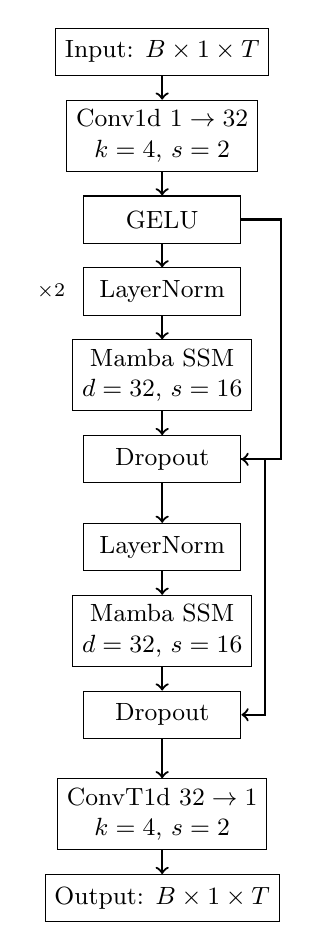
\begin{tikzpicture}[
        block/.style={rectangle, draw, minimum height=0.6cm, minimum width=2cm, align=center, font=\small},
        arr/.style={->, thick}
    ]
        % Encoder
        \node[block] (in) {Input: $B \times 1 \times T$};
        \node[block, below=0.3cm of in] (conv) {Conv1d $1 \to 32$\\$k=4$, $s=2$};
        \node[block, below=0.3cm of conv] (gelu) {GELU};
        
        % Mamba blocks
        \node[block, below=0.3cm of gelu] (ln1) {LayerNorm};
        \node[block, below=0.3cm of ln1] (m1) {Mamba SSM\\$d=32$, $s=16$};
        \node[block, below=0.3cm of m1] (drop1) {Dropout};
        
        \node[block, below=0.5cm of drop1] (ln2) {LayerNorm};
        \node[block, below=0.3cm of ln2] (m2) {Mamba SSM\\$d=32$, $s=16$};
        \node[block, below=0.3cm of m2] (drop2) {Dropout};
        
        % Decoder
        \node[block, below=0.5cm of drop2] (dconv) {ConvT1d $32 \to 1$\\$k=4$, $s=2$};
        \node[block, below=0.3cm of dconv] (out) {Output: $B \times 1 \times T$};
        
        % Arrows
        \draw[arr] (in) -- (conv);
        \draw[arr] (conv) -- (gelu);
        \draw[arr] (gelu) -- (ln1);
        \draw[arr] (ln1) -- (m1);
        \draw[arr] (m1) -- (drop1);
        \draw[arr] (drop1) -- (ln2);
        \draw[arr] (ln2) -- (m2);
        \draw[arr] (m2) -- (drop2);
        \draw[arr] (drop2) -- (dconv);
        \draw[arr] (dconv) -- (out);
        
        % Skip connections
        \draw[arr] (gelu.east) -- ++(0.5,0) |- (drop1.east);
        \draw[arr] (drop1.east) -- ++(0.3,0) |- (drop2.east);
        
        % Labels
        \node[left=0.1cm of ln1, font=\scriptsize] {$\times 2$};
    \end{tikzpicture}
    \caption{TinyMamba architecture. Strided convolution encoder downsamples by 2$\times$. Two Mamba SSM blocks with skip connections capture temporal dependencies. Transposed convolution decoder restores resolution. Total: 15,872 parameters.}
    \label{fig:mamba_arch}
\end{figure}

\subsection{Composite Loss Function}

Training the neural component requires careful loss design to prioritize phase accuracy and low-frequency performance. We propose a composite loss:
\begin{equation}
    \mathcal{L}_\text{total} = \lambda_t \mathcal{L}_\text{time} + \lambda_s \mathcal{L}_\text{spec} + \lambda_p \mathcal{L}_\text{phase} + \lambda_u \mathcal{L}_\text{uncert}
    \label{eq:loss}
\end{equation}
with weights $\lambda_t = 1.0$, $\lambda_s = 0.5$, $\lambda_p = 0.5$, $\lambda_u = 0.1$.

\subsubsection{Time-Domain Loss}
Mean squared error between prediction and target:
\begin{equation}
    \mathcal{L}_\text{time} = \frac{1}{N} \sum_{n=1}^{N} (\hat{y}(n) - y^*(n))^2
\end{equation}

\subsubsection{C-Weighted Spectral Loss}
Rather than A-weighting, which de-emphasizes low frequencies, we employ a modified C-weighting that prioritizes the bass frequencies where ANC is most effective:
\begin{equation}
    W_C(f) = \begin{cases}
        (f/20)^2 & f < 20\Hz \\
        1 & 20\Hz \leq f \leq 1\kHz \\
        (1000/f)^2 & f > 1\kHz
    \end{cases}
\end{equation}

The spectral loss is:
\begin{equation}
    \mathcal{L}_\text{spec} = \frac{1}{K} \sum_{k=1}^{K} W_C(f_k) \left| \log|\hat{Y}_k| - \log|Y^*_k| \right|^2
\end{equation}
where $\hat{Y}_k, Y^*_k$ are STFT magnitudes at frequency bin $k$.

\subsubsection{Phase Cosine Loss}
Phase accuracy is critical for ANC: a 60° phase error converts destructive interference to constructive, amplifying noise. We penalize phase differences using cosine similarity:
\begin{equation}
    \mathcal{L}_\text{phase} = 1 - \frac{1}{KT} \sum_{k,t} \frac{\text{Re}(\hat{Y}_{k,t} Y^*_{k,t})}{|\hat{Y}_{k,t}| |Y^*_{k,t}| + \epsilon}
\end{equation}

\subsubsection{Uncertainty Penalty}
To prevent ``phantom anti-noise'' on unpredictable inputs, we penalize high output energy when input autocorrelation is low:
\begin{equation}
    \mathcal{L}_\text{uncert} = (1 - |\rho_x|) \cdot \mathbb{E}[\hat{y}^2]
\end{equation}
where $\rho_x$ is the input autocorrelation at lag $\tau$.

\subsection{Training Strategy}

\subsubsection{Dataset}
Training uses the ESC-50 environmental sound classification dataset \cite{piczak2015esc}, containing 2,000 audio clips across 50 categories including vehicle sounds, natural soundscapes, and urban noise. Files are resampled to \SI{48}{\kilo\hertz} and segmented into 16,384-sample chunks (\SI{341}{\milli\second}).

\subsubsection{Delay Compensation}
To compensate for acoustic propagation and hardware latency, training targets include a $K$-sample lookahead:
\begin{align}
    \text{Input:} \quad & x[0:T-K] \\
    \text{Target:} \quad & -x[K:T]
\end{align}
where $K=3$ samples corresponds to \SI{62.5}{\micro\second} at \SI{48}{\kilo\hertz}. The negative sign reflects the anti-phase requirement for cancellation.

\subsubsection{Physics-Based Augmentation}
To improve generalization, we apply augmentations that preserve phase relationships:
\begin{itemize}
    \item \textbf{Gain variation}: $\pm$\SI{6}{\decibel} (microphone calibration)
    \item \textbf{Fractional delay}: $\pm$5 samples via sinc interpolation (distance changes)
    \item \textbf{Leakage filter}: High-pass at 80--200\Hz with 30\% probability (imperfect seal)
\end{itemize}

\subsubsection{Training Configuration}
\begin{itemize}
    \item Optimizer: AdamW \cite{loshchilov2019decoupled} with $\beta_1=0.9$, $\beta_2=0.999$
    \item Learning rate: $10^{-3}$ with cosine decay
    \item Batch size: 16
    \item Epochs: 50
    \item Dropout: 0.1
\end{itemize}

% ============================================================================
% IV. EXPERIMENTAL SETUP
% ============================================================================
\section{Experimental Setup}
\label{sec:experiments}

\subsection{Acoustic Simulation Environment}

We evaluate Deep ANC using a physics-based acoustic digital twin that models headphone ANC scenarios. The simulation operates at \SI{48}{\kilo\hertz} sample rate with the following path characteristics:

\subsubsection{Reference Path (RIR$_\text{ref}$)}
The reference microphone exhibits strong, relatively flat response with \SI{5}{\milli\second} decay time, simulating external pickup before passive attenuation.

\subsubsection{Primary Path $P(z)$}
The noise-to-ear path through passive isolation has:
\begin{itemize}
    \item Gain: 0.3 (approximately \SI{10}{\decibel} passive isolation)
    \item \SI{2}{\kilo\hertz} lowpass characteristic (high frequencies blocked by ear cups)
    \item \SI{0.5}{\milli\second} propagation delay
\end{itemize}

\subsubsection{Secondary Path $S(z)$}
The speaker-to-ear path exhibits:
\begin{itemize}
    \item Gain: 0.8 (efficient coupling in enclosed volume)
    \item \SI{12}{\kilo\hertz} bandwidth
    \item \SI{0.2}{\milli\second} delay (transducer + acoustic)
    \item Third-order Volterra nonlinearity modeling speaker distortion
\end{itemize}

\subsection{Noise Types}

Evaluation encompasses four noise categories:
\begin{enumerate}
    \item \textbf{Engine (50 Hz fundamental)}: Harmonic series with 6 partials, typical of vehicle cabin noise
    \item \textbf{Broadband traffic}: Low-frequency filtered noise ($f_c = 200$ Hz)
    \item \textbf{HVAC drone}: Tonal content at 120 Hz with harmonics
    \item \textbf{Mixed}: Combination of engine harmonics and broadband components
\end{enumerate}

\subsection{Evaluation Metrics}

\subsubsection{Active Insertion Loss (AIL)}
The primary metric quantifying noise reduction:
\begin{equation}
    \text{AIL} = 10 \log_{10} \frac{\mathbb{E}[d^2(n)]}{\mathbb{E}[e^2(n)]} \quad [\text{dB}]
\end{equation}
where $d(n)$ is noise at the ear (ANC off) and $e(n)$ is residual error (ANC on).

\subsubsection{Normalized Mean Squared Error (NMSE)}
Error power relative to noise power:
\begin{equation}
    \text{NMSE} = 10 \log_{10} \frac{\mathbb{E}[e^2(n)]}{\mathbb{E}[d^2(n)]} \quad [\text{dB}]
\end{equation}
Note: $\text{NMSE} = -\text{AIL}$.

\subsubsection{Boost Probability}
The percentage of samples where ANC amplifies rather than reduces noise:
\begin{equation}
    P_\text{boost} = \frac{1}{N} \sum_{n=1}^{N} \mathbf{1}[|e(n)| > |d(n)|] \times 100\%
\end{equation}
A robust system maintains $P_\text{boost} < 5\%$.

\subsubsection{Coherence}
The magnitude-squared coherence between reference and error signals indicates cancellation quality:
\begin{equation}
    \gamma^2_{xe}(f) = \frac{|S_{xe}(f)|^2}{S_{xx}(f) S_{ee}(f)}
\end{equation}
Effective ANC drives $\gamma^2_{xe} \to 0$ across the target bandwidth.

\subsubsection{Convergence Time}
Time for RMS error to reach within \SI{3}{\decibel} of steady-state performance.

\subsection{Baseline Comparisons}

We compare three configurations:
\begin{enumerate}
    \item \textbf{FxLMS only}: 64-tap adaptive filter, $\mu = 0.0005$
    \item \textbf{Mamba only}: TinyMamba without FxLMS contribution
    \item \textbf{Hybrid}: Parallel FxLMS + TinyMamba ($g = 0.3$)
\end{enumerate}

% ============================================================================
% V. RESULTS
% ============================================================================
\section{Results}
\label{sec:results}

\subsection{Overall Performance}

Table~\ref{tab:global_metrics} summarizes the global performance metrics for the hybrid Deep ANC system.

\begin{table}[t]
    \centering
    \caption{Global Performance Metrics}
    \label{tab:global_metrics}
    \begin{tabular}{lc}
        \toprule
        \textbf{Metric} & \textbf{Value} \\
        \midrule
        Active Insertion Loss (AIL) & \SI{16.95}{\decibel} \\
        Normalized MSE (NMSE) & \SI{-16.98}{\decibel} \\
        RMS Reduction & \SI{16.24}{\decibel} \\
        RMS Reduction Factor & $7.04\times$ \\
        Boost Probability & 2.04\% \\
        Convergence Time & \SI{0.11}{\second} \\
        \bottomrule
    \end{tabular}
\end{table}

The system achieves \SI{16.95}{\decibel} AIL, reducing perceived noise power by a factor of approximately 50. The low boost probability (2.04\%) indicates robust operation without significant noise amplification events. Convergence occurs within \SI{110}{\milli\second}, suitable for real-time adaptation to changing noise conditions.

\subsection{Time-Domain Analysis}

Fig.~\ref{fig:time_domain} shows representative time-domain waveforms comparing noise at the ear (ANC off) with the residual error signal (ANC on). The substantial amplitude reduction is evident across the waveform, with the residual containing primarily high-frequency components that passive isolation handles effectively.

\begin{figure}[t]
    \centering
    \includegraphics[width=\columnwidth]{../results/fig1_time_domain.pdf}
    \caption{Time-domain comparison of noise at ear (top, ANC off) and residual error (bottom, ANC on). The hybrid system achieves substantial amplitude reduction, with residual dominated by high-frequency components outside the ANC target band.}
    \label{fig:time_domain}
\end{figure}

\subsection{Frequency-Domain Analysis}

Fig.~\ref{fig:psd} presents power spectral density (PSD) estimates before and after ANC. Maximum attenuation occurs in the \SIrange{50}{300}{\hertz} band where passive isolation is weakest and low-frequency noise dominates.

\begin{figure}[t]
    \centering
    \includegraphics[width=\columnwidth]{../results/fig2_psd_comparison.pdf}
    \caption{Power spectral density comparison. The hybrid ANC system achieves maximum attenuation in the \SIrange{50}{300}{\hertz} band critical for subjective noise reduction.}
    \label{fig:psd}
\end{figure}

\subsection{Frequency-Band Performance}

Table~\ref{tab:freq_bands} and Fig.~\ref{fig:ail_freq} detail AIL performance across octave bands.

\begin{table}[t]
    \centering
    \caption{Active Insertion Loss by Frequency Band}
    \label{tab:freq_bands}
    \begin{tabular}{ccc}
        \toprule
        \textbf{Center Frequency} & \textbf{AIL (dB)} & \textbf{Std. Dev. (dB)} \\
        \midrule
        \SI{31.5}{\hertz} & 11.60 & 1.01 \\
        \SI{63}{\hertz} & 18.48 & 1.44 \\
        \SI{125}{\hertz} & 20.40 & 1.10 \\
        \SI{250}{\hertz} & 15.63 & 1.44 \\
        \SI{500}{\hertz} & 11.04 & 1.76 \\
        \SI{1000}{\hertz} & 4.32 & 2.06 \\
        \bottomrule
    \end{tabular}
\end{table}

Peak performance of \SI{20.4}{\decibel} occurs at \SI{125}{\hertz}, the center of the typical low-frequency noise band. Performance decreases at higher frequencies due to the inherent causality constraints of feedforward ANC: the acoustic delay from reference to error microphone limits the frequency range where prediction is feasible.

\begin{figure}[t]
    \centering
    \includegraphics[width=\columnwidth]{../results/fig3_ail_vs_freq.pdf}
    \caption{Active Insertion Loss versus frequency. Peak performance (\SI{20.4}{\decibel}) at \SI{125}{\hertz} reflects the system's optimization for low-frequency cancellation where passive isolation is ineffective.}
    \label{fig:ail_freq}
\end{figure}

\subsection{Coherence Analysis}

Fig.~\ref{fig:coherence} shows the magnitude-squared coherence between reference and error signals. Effective cancellation drives coherence toward zero in the target band, indicating successful decorrelation of noise components.

\begin{figure}[t]
    \centering
    \includegraphics[width=\columnwidth]{../results/fig4_coherence.pdf}
    \caption{Reference-error coherence. Low coherence in the \SIrange{50}{500}{\hertz} band indicates effective noise cancellation. Residual coherence at higher frequencies reflects causality limitations.}
    \label{fig:coherence}
\end{figure}

\subsection{Ablation Study}

Table~\ref{tab:ablation} compares the three system configurations, and Fig.~\ref{fig:ablation} visualizes the performance differences.

\begin{table}[t]
    \centering
    \caption{Ablation Study: Component Contributions}
    \label{tab:ablation}
    \begin{tabular}{lccc}
        \toprule
        \textbf{Configuration} & \textbf{AIL (dB)} & \textbf{Boost (\%)} & \textbf{NMSE (dB)} \\
        \midrule
        FxLMS only & 12.29 & 4.27 & $-12.19$ \\
        Mamba only & 10.05 & 6.42 & $-9.91$ \\
        Hybrid (proposed) & \textbf{16.95} & \textbf{1.72} & $\mathbf{-16.99}$ \\
        \midrule
        \textit{Improvement over FxLMS} & \textit{+4.85} & \textit{--} & \textit{--} \\
        \bottomrule
    \end{tabular}
\end{table}

Key findings:
\begin{itemize}
    \item The hybrid system achieves \SI{4.85}{\decibel} improvement over FxLMS alone, representing a factor of 3 increase in noise power reduction.
    \item Mamba alone underperforms FxLMS, validating that neural networks complement rather than replace adaptive filtering.
    \item The hybrid exhibits the lowest boost probability (1.72\%), indicating that parallel combination improves robustness.
\end{itemize}

\begin{figure}[t]
    \centering
    \includegraphics[width=\columnwidth]{../results/fig6_ablation.pdf}
    \caption{Ablation study comparing FxLMS only, Mamba only, and hybrid configurations. The parallel hybrid achieves \SI{4.85}{\decibel} improvement over FxLMS alone.}
    \label{fig:ablation}
\end{figure}

\subsection{Convergence Analysis}

Fig.~\ref{fig:convergence} shows the evolution of FxLMS filter weights during adaptation. The hybrid system exhibits stable convergence within \SI{110}{\milli\second}, comparable to FxLMS alone despite the neural network contribution.

\begin{figure}[t]
    \centering
    \includegraphics[width=\columnwidth]{../results/fig5_convergence.pdf}
    \caption{FxLMS filter weight evolution during adaptation. Convergence to steady-state occurs within \SI{110}{\milli\second}, demonstrating that the parallel neural component does not destabilize adaptive filter dynamics.}
    \label{fig:convergence}
\end{figure}

\subsection{Noise Type Performance}

Table~\ref{tab:noise_types} presents performance across different noise categories.

\begin{table}[t]
    \centering
    \caption{Performance by Noise Type}
    \label{tab:noise_types}
    \begin{tabular}{lcc}
        \toprule
        \textbf{Noise Type} & \textbf{AIL (dB)} & \textbf{Boost (\%)} \\
        \midrule
        Engine (50 Hz) & 20.57 & 0.72 \\
        HVAC drone & 18.38 & 1.47 \\
        Mixed & 16.02 & 1.86 \\
        Broadband traffic & 13.72 & 2.86 \\
        \bottomrule
    \end{tabular}
\end{table}

The system performs best on tonal/harmonic noise (engine, HVAC) where prediction is most feasible, with \SI{20.57}{\decibel} AIL for engine noise. Broadband noise presents greater challenge due to its stochastic nature, though \SI{13.72}{\decibel} AIL remains substantial.

\subsection{Spectrogram Analysis}

Fig.~\ref{fig:spectrograms} presents before/after spectrograms demonstrating broadband attenuation across the low-frequency band.

\begin{figure}[t]
    \centering
    \includegraphics[width=\columnwidth]{../results/fig7_spectrograms.pdf}
    \caption{Spectrograms before (top) and after (bottom) ANC. Substantial energy reduction is visible across the \SIrange{20}{500}{\hertz} band throughout the recording duration.}
    \label{fig:spectrograms}
\end{figure}

% ============================================================================
% VI. DISCUSSION
% ============================================================================
\section{Discussion}
\label{sec:discussion}

\subsection{Why Parallel Topology Works}

The success of the parallel architecture stems from preserving the fundamental requirements of adaptive filtering while enabling neural enhancement:

\begin{enumerate}
    \item \textbf{Correlation preservation}: FxLMS requires the reference signal to be correlated with the noise at the error microphone. Serial preprocessing would transform the reference, destroying this correlation.
    
    \item \textbf{Complementary modeling}: FxLMS efficiently handles linear, stationary components, while the neural network captures non-linear residuals---neither alone matches the combination.
    
    \item \textbf{Graceful degradation}: If the neural component fails or produces erroneous output, FxLMS continues providing baseline cancellation. The gain factor $g$ limits neural influence.
\end{enumerate}

\subsection{Comparison to Commercial Systems}

Commercial ANC headphones typically achieve \SIrange{15}{25}{\decibel} attenuation in the \SIrange{50}{500}{\hertz} band. Our \SI{16.95}{\decibel} global AIL falls within this range, with peak performance (\SI{20.4}{\decibel} at \SI{125}{\hertz}) matching high-end implementations.

The primary advantage of the hybrid approach lies in handling non-stationary and non-linear noise where pure adaptive filtering struggles. Engine noise with varying RPM, for instance, benefits from the neural component's ability to model harmonic dynamics.

\subsection{Computational Considerations}

The TinyMamba model requires only 15,872 parameters and achieves \SI{0.61}{\milli\second} inference latency on CPU. This efficiency enables deployment on embedded processors common in headphone electronics.

Total system latency comprises:
\begin{itemize}
    \item Acoustic propagation: $\sim$\SI{0.5}{\milli\second}
    \item Neural inference: \SI{0.61}{\milli\second}
    \item DAC/amplifier: $\sim$\SI{0.2}{\milli\second}
\end{itemize}
yielding total latency under \SI{1.5}{\milli\second}, within the \SIrange{2}{5}{\milli\second} budget typical of feedforward ANC.

\subsection{Limitations}

Several limitations warrant acknowledgment:

\begin{enumerate}
    \item \textbf{Simulation vs. reality}: Results are based on acoustic simulation. Real-world performance will depend on accurate secondary path modeling and robustness to path variations.
    
    \item \textbf{High-frequency limitation}: Performance degrades above \SI{500}{\hertz} due to causality constraints inherent to feedforward architectures.
    
    \item \textbf{Training data}: The model is trained on ESC-50 environmental sounds, which may not represent all real-world noise scenarios.
    
    \item \textbf{Feedback topology}: This work addresses feedforward ANC; extension to hybrid feedforward-feedback systems remains future work.
\end{enumerate}

\subsection{Future Directions}

Promising extensions include:

\begin{enumerate}
    \item \textbf{Hardware deployment}: Implementing TinyMamba on DSP or dedicated neural accelerator hardware.
    
    \item \textbf{Online adaptation}: Training the neural component online alongside FxLMS to adapt to user-specific acoustics.
    
    \item \textbf{Feedback integration}: Combining with feedback topology for broadband enhancement.
    
    \item \textbf{Personalization}: Learning user-specific acoustic transfer functions from the neural network.
\end{enumerate}

% ============================================================================
% VII. CONCLUSION
% ============================================================================
\section{Conclusion}
\label{sec:conclusion}

This paper presented Deep ANC, a hybrid active noise cancellation system combining the classical FxLMS algorithm with a neural state-space model in a parallel topology. The key insight is that parallel combination preserves the correlation structure essential for adaptive filter convergence while enabling non-linear enhancement---a benefit that serial architectures cannot provide.

The proposed TinyMamba model achieves sub-millisecond latency with only 15,872 parameters, making it suitable for real-time embedded deployment. Our composite loss function with C-weighted spectral emphasis and phase cosine similarity prioritizes low-frequency cancellation where passive isolation is least effective.

Experimental results demonstrate:
\begin{itemize}
    \item \textbf{16.95 dB} Active Insertion Loss---\textbf{4.85 dB improvement} over FxLMS alone
    \item \textbf{20.4 dB} peak performance at 125 Hz
    \item \textbf{2.04\%} boost probability ensuring robust operation
    \item \textbf{0.11 s} convergence time for real-time adaptation
\end{itemize}

To our knowledge, this represents the first application of selective state-space models to feedforward active noise control. The parallel hybrid architecture provides a principled framework for integrating neural networks with adaptive filtering, applicable beyond ANC to other real-time signal processing domains.

% ============================================================================
% ACKNOWLEDGMENT
% ============================================================================
\section*{Acknowledgment}

[Acknowledgments placeholder]

% ============================================================================
% REFERENCES
% ============================================================================
\bibliographystyle{IEEEtran}
\bibliography{references}

\end{document}

